\documentclass[TechnicalNoteMeteo.tex]{subfiles}

\begin{document}

The algorithm described in this paper is based on the classical MLR (Multiple Linear Regression) method presented in \cite{eischeid_creating_2000}. The MLR method is a robust and well known spatial interpolation technique that can indirectly account for local effects, such as topography, land cover, land use and surface water. While creating serially complete daily datasets of air temperature and total precipitation for the western U.S., \cite{eischeid_creating_2000} found that the MLR method consistently outperformed the other classical methods tested (normal ratio, inverse distance, optimal interpolation, and single best estimator). The same result was also found by \cite{xia_forest_1999} for a study in Bavaria, Germany. Moreover, in a study conducted in Iran for different climate conditions (dry to extra humid conditions), \cite{kashani_evaluation_2011} found that the estimation obtained with the MLR method compared well with those obtained with more recent methods, more specifically the artificial neural network (reference) and the genetic programming (references) techniques.

A flowchart of our gap-filling algorithm is shown in \cref{fig:fillworker_flowchart}. The algorithm consists of two nested loops: the external `Loop A' iterates over the weather variables of the dataset (min, max, and mean air temperature and total precipitation), while the inner `Loop B' iterates over the missing values in each weather data series. Each missing value is estimated independently with a two-step procedure in `Loop B'. The first step consists in the selection of the neighboring stations. The second step consists in building a MLR model, estimating the missing value, and filling the corresponding gap in the data series. The gap-filling algorithm of \cref{fig:fillworker_flowchart} is described in more details in the following sections of this paper.

\begin{figure}[!p]
    \centering
    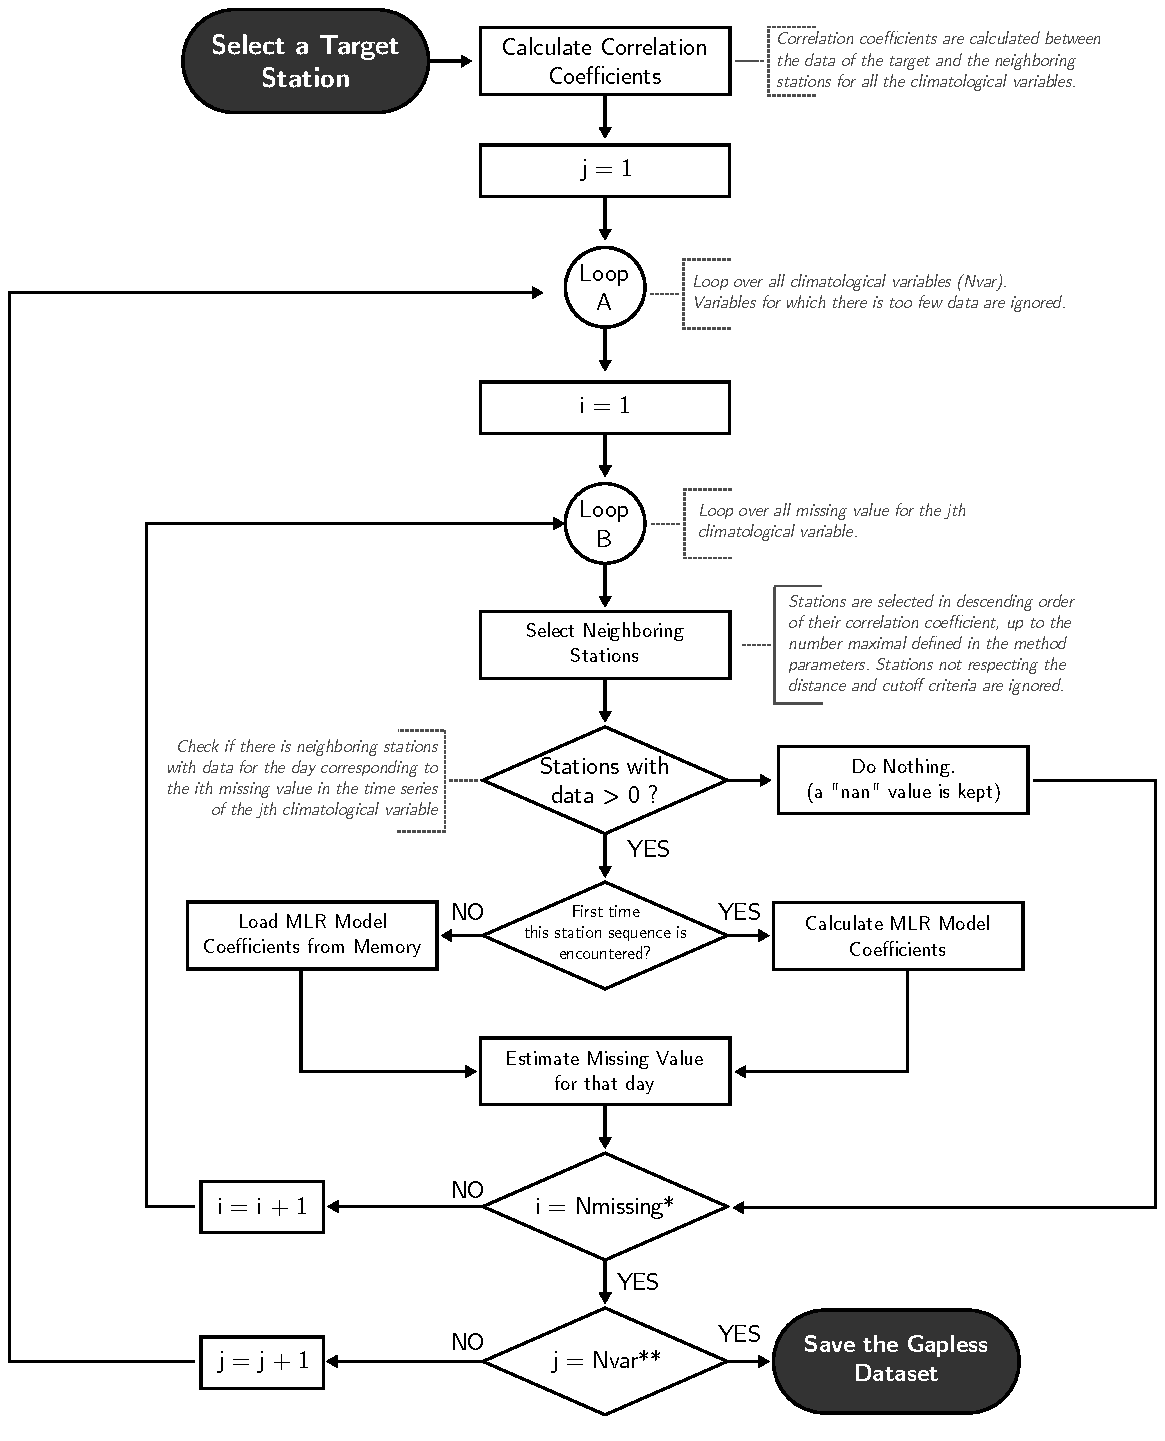
\includegraphics[width=\textwidth]{img/Flowchart-filling_missing_weather.pdf} 
    \caption{}
    \label{fig:fillworker_flowchart}
\end{figure}

\subsection{Correlation Coefficients Calculations}

Correlation coefficients are calculated between the available data of the target station and those of the neighboring stations for each weather variable individually. The coefficients are calculated using all the available data. However, neighboring stations that have less than 182 days (half a year) of synchronous data with the target station or that have a correlation coefficient below a value of 0.35, for a given weather variable, are not used to fill the gaps in the data for that weather variable. The 0.35 threshold is based on the value used by \cite{eischeid_creating_2000} in their application of the method. 

Moreover, it is possible to discard completely from the gap-filling procedure neighboring stations that are located farther away from the target station than specified thresholds, either in the horizontal or the vertical direction. The default values are set to \SI{100}{km} and \SI{350}{m} for the horizontal and vertical distance respectively, based on the values found in the literature \citep{tronci_comparison_1986,xia_forest_1999,simolo_improving_2010}.

\subsection{Selection of the Neighboring Stations}\label{sec:select_stations}

As stated by \cite{eischeid_creating_2000}, the selection of neighboring stations is critically important for the accurate estimation of missing weather data. Problems arise though because the set of neighboring stations with available data can vary from one day to the other. Therefore, the process of selecting the neighboring stations for the generation of a MLR model is repeated for each missing value in the dataset of the target station. 

The neighboring stations with available data are selected in descending order of their correlation coefficient, up to a maximal number of stations that can be specified as a parameter in the algorithm. The default value for the maximal number of neighboring stations used for the generation of the MLR models is 4. Tests run by \cite{eischeid_creating_2000} showed that using more then 4 neighboring stations did not significantly improve, and may even have degraded, the accuracy of the estimates. If for a given day with a missing value, no neighboring stations have a measured value, no calculation is done and a ‘NaN' value is kept in the dataset. 

\subsection{Generation of the Multiple Linear Regression Model}\label{subsec:MLR_gen}

Each time a MLR model is generated for a given sequence of neighboring stations, the result is stored into memory. Therefore, after a set of neighboring stations have been selected for a given day where a data is missing (\cref{sec:select_stations}), the program checks first if this sequence of stations has already been encountered before for the current weather variable. If so, the stored MLR parameters will be used directly to estimate the missing data for the current day. Otherwise, a new MLR model will be generated from the newly encountered set of neighboring stations to estimate the missing data. Since a MLR model is generated only once for a given sequence of neighboring stations, the algorithm becomes faster with time as the number of MLR models stored into memory increases.

The MLR models can be generated using either an Ordinary Least Square~(OLS) or a Least Absolute Deviations~(LAD) criteria. Since daily precipitation series are generally characterized by long-tailed and positively skewed distributions, the LAD method is more appropriate than the OLS method since it is more robust to outliers \citep{menke_geophysical_1989,eischeid_creating_2000}. The downside in using the LAD method is an increase in computation time by about a factor 10 compared to the OLS method. The resolution of the MLR models with the LAD method is achieved using an iterative reweighted least-squares method (reference).

%https://en.wikipedia.org/wiki/Iteratively_reweighted_least_squares


\subsection{Estimating Missing Daily Values}\label{sec:est_miss_values}

The value of the weather data for the target station is estimated from the synchronous measurements of the neighboring stations using the MLR model, such as:
%
\begin{equation}
    Y_{t} = a_0 + \sum_{k=1}^{N} a_k \cdot X_k(t_i)
\end{equation}
%
where $Y(t)$ is the value estimated for the target station at time $t$, $X_k(t)$ is the synchronous measured data for the $k^{th}$ neighboring stations, $a_k$ are the regression coefficients of the MLR model, and $N$ is the total number of neighboring stations that were used for the regression. The intercept term, $a_0$, is estimated for the air temperature, but is set to zero for precipitation. 

It is possible to have a negative regression coefficients for the less correlated neighboring stations used to generate the MLR model. If so, the MLR model will sometimes yield small negative values for daily precipitation. To correct that, negative values estimated for daily precipitation are always set to zero.

\subsection{Uncertainty of the estimated values}\label{subsec:crossval}

The accuracy of each MLR model generated throughout the gap-filling procedure is estimated by computing the root mean of squared residuals of the regression. It is also possible to evaluate the accuracy of the whole method (instead of each MLR model individually) for the entire dataset of given weather station with a Leave One Out (LOO) cross-validation procedure. The procedure consists in estimating a value for each day of the data series of each weather variable for which a measured data is available in the dataset (in addition to the days with missing data). In other words, the loops A and B in the flowchart of \cref{fig:fillworker_flowchart} iterates over all the days and all the weather variables of the dataset instead of only iterating over days with a missing data. Before estimating a value for a given day, the corresponding measured data is temporarily discarded from the dataset of the target station to avoid self-influence of this observation on the generation of the MLR model. The accuracy of the method is then estimated by computing the Root-Mean-Square Error (RMSE), the Mean-Absolute Error (MAE), the Mean Error (ME) and the correlation coefficient~(r) between the estimated weather data and the respective non-missing observations in the original dataset of the target station.

Since a new MLR model must be generated for each day independently when doing the cross-validation procedure, the computation time of the gap-filling procedure is thus significantly increased. This is especially true if the MLR model is generated with the least absolute deviation regression method. For this reason, the cross-validation procedure is by default not activated in the algorithm.

\end{document}

%This is done by using the model to estimate a value for each day in the data series of the target station for which a measured value exists and for which the neighboring stations have data. The accuracy of the MLR model is then approximated by computing the Root-Mean-Square Error (RMSE) between the estimated values and the respective observations in the data series of the target station.

%Though costly in computation time, enabling this option can provide interesting insights on the performance of the procedure for the specific datasets used for a given project.


%For the OLS criteria, the MLR models are obtained by solving the linear matrix equation $\mathbf{X}\mathbf{a} = \mathbf{Y}$ by computing the $N \times 1$ parameter vector $\mathbf{a}$ that minimizes the Euclidean L2-norm $\left\Vert \mathbf{Y}-\mathbf{X}\mathbf{a} \right\Vert_2$, where $\mathbf{Y}$ is a $M \times 1$ vector containing the M daily data of the target station and $\mathbf{X}$ is a $M \times N$ matrix containing the M synchronous daily data of the N selected neighboring stations. (REFERENCE: Numpy Documentation)

%Essentially, the classifier is trained on a subset of the training data set, and tested on the remainder. This process is repeated systematically so that all the points in the training set are tested.

%Cross-validation is a way to predict the fit of a model to a hypothetical validation set when an explicit validation set is not available.

%\subsubsection{Quality Control}

%the correlation between the data of the neighboring and target stations will generally decrease as the horizontal distance and elevation difference between them increase. Therefore,

%It is not possible to use a single MLR model to estimate the missing values in the dataset of the target station all at once.
 
%Prior to the analysis of weather time series, it is important to apply quality control constraints to ensure that the data do not violate obvious constraints associated with minimum, maximum, and average daily air temperature and daily cumulative precipitation. 

%The program will identify irregularities or inconsistencies to insure that maximum, minimum and average daily temperatures are coherent for a given day and that all daily precipitation values are positive. Erroneous values are replaced by nan values in the dataset. These values will subsequently be estimated by the program from neighboring stations.

%Among these techniques, methods based on the use of data from neighboring stations are generally favored to within-station methods, i.e. those that only use data from the series being filled.

%have been proven to perform poorly compared to methods based on the use of data from neighboring stations for the reconstruction of daily precipitation time series (Eischeid et al., 1995; Kemp et al., 1983; Simolo et al., 2010).

%The creation of a serially complete weather dataset generally consists in the replacement of missing daily data with estimated values calculated from simultaneous observations at nearby stations. 

%Numerous spatial interpolation techniques exist for handling the missing data in the weather time series of a given station by using data from irregularly spaced neighboring station (e.g. simple arithmetic averaging, inverse distance method, single best estimator and multiple regression analysis).

% An example of this problem is illustrated in \cref{tab:selectStations}, where theoretical time-series of air temperature data are presented. In this example, there are missing values in the dataset of the target station, Y, for days 2, 4, and 5. Therefore, the missing value on day 2 will be estimated with data from the neighboring stations X1, X3, and X4 since there is also a missing value on this day for station X2. All neighboring stations will be used for the estimation of the missing value on day 4. Finally, only stations X1 and X2 will be used for the estimation of the missing value on day 5.
%
%\begin{table}[!hb]
%\newcommand{\nan}{\multicolumn{1}{c}{\textbf{nan}}}
%\center
%\caption{This table shows some data}
%\begin{tabular}{
%S[table-format = 1]
%*5S[table-format = 2.1]
%}
%\toprule
%& {Target} & \multicolumn{4}{c}{Neighbors} \\
%\cmidrule(lr){3-6}
%{Day} & {Y} & {X1} & {X2} & {X3} & {X4} \\
%\midrule
%%\rowcolor{gray!30}
%1 & 11.0 & 12.0 & 12.0 & 12.5 & 10.0 \\
%2 & \nan & 12.0 & \nan & 13.0 & 12.2 \\
%3 &   7.5 &  8.5 &   8.5 &  8.0 &  8.9 \\
%4 & \nan &  6.0 &   4.5 &  5.0 &  4.4 \\
%5 & \nan &  8.0 &   8.5 & \nan & \nan \\
%\bottomrule
%\end{tabular}
%\label{tab:selectStations}
%\end{table}
